\documentclass[11pt,a4paper]{article}

% ---------------------------------------------------------------------------
% Packages
% ---------------------------------------------------------------------------
\usepackage[a4paper,margin=2.5cm]{geometry}
\usepackage[utf8]{inputenc}
\usepackage[T1]{fontenc}
\usepackage{graphicx}
\usepackage{xcolor}
\usepackage{booktabs}
\usepackage{longtable}
\usepackage{array}
\usepackage{listings}
\usepackage{tikz}
\usetikzlibrary{positioning,fit,arrows.meta,calc}
\usepackage{amsmath}
\usepackage{hyperref}
\usepackage{caption}
\usepackage{enumitem}
\usepackage{fancyhdr}
\usepackage{titlesec}

\graphicspath{{./figures/}}

% ---------------------------------------------------------------------------
% Colors
% ---------------------------------------------------------------------------
\definecolor{codebg}{rgb}{0.97,0.97,0.97}
\definecolor{codekw}{rgb}{0.0,0.0,0.6}
\definecolor{codecom}{rgb}{0.35,0.55,0.35}
\definecolor{codestr}{rgb}{0.6,0.1,0.1}
\definecolor{michwarblue}{HTML}{4C72B0}
\definecolor{michwarorange}{HTML}{DD8452}

% ---------------------------------------------------------------------------
% Listings setup
% ---------------------------------------------------------------------------
\lstdefinelanguage{Dart}{
  keywords={abstract, async, await, class, const, enum, extends, final, Future,
    get, import, library, return, set, static, Stream, this, throw, try,
    catch, void, var, new, required, implements, with, on, as, is, in, for,
    while, do, if, else, switch, case, break, continue, default, null, true,
    false, late, factory, mixin, typedef, yield, export, part, show, hide,
    dynamic},
  sensitive=true,
  morecomment=[l]{//},
  morecomment=[s]{/*}{*/},
  morestring=[b]",
  morestring=[b]',
}

\lstdefinelanguage{JSPB}{
  keywords={function, var, return, if, else, for, while, new, throw, try,
    catch, true, false, null, this, typeof, instanceof, in, of, break,
    continue, const, let},
  sensitive=true,
  morecomment=[l]{//},
  morecomment=[s]{/*}{*/},
  morestring=[b]",
  morestring=[b]',
}

\lstset{
  basicstyle=\ttfamily\footnotesize,
  backgroundcolor=\color{codebg},
  keywordstyle=\color{codekw}\bfseries,
  commentstyle=\color{codecom}\itshape,
  stringstyle=\color{codestr},
  numbers=left,
  numberstyle=\tiny\color{gray},
  numbersep=8pt,
  breaklines=true,
  breakatwhitespace=false,
  showstringspaces=false,
  frame=single,
  rulecolor=\color{gray!40},
  framerule=0.4pt,
  tabsize=2,
  captionpos=b,
  xleftmargin=1em,
  framexleftmargin=1.2em,
}

% Convenient inline code macro (verbatim-safe: handles _, $, {, } etc.)
\newcommand{\code}[1]{\lstinline[basicstyle=\ttfamily\small]{#1}}

% ---------------------------------------------------------------------------
% Header / footer
% ---------------------------------------------------------------------------
\pagestyle{fancy}
\setlength{\headheight}{14pt}
\fancyhf{}
\fancyhead[L]{MICHWAR --- Self-Hosted Ride-Hailing Platform}
\fancyhead[R]{\thepage}
\renewcommand{\headrulewidth}{0.3pt}

\titleformat{\section}{\normalfont\Large\bfseries}{\thesection}{1em}{}
\titleformat{\subsection}{\normalfont\large\bfseries}{\thesubsection}{1em}{}

% ---------------------------------------------------------------------------
% Title
% ---------------------------------------------------------------------------
\title{
  \vspace{-1.5cm}
  \rule{\linewidth}{0.5pt}\\[0.4cm]
  {\Huge \textbf{MICHWAR}}\\[0.3cm]
  {\Large Design, Migration, and Deployment of a Self-Hosted Backend\\
   for a Ride-Hailing Platform}\\[0.3cm]
  \rule{\linewidth}{0.5pt}\\[0.6cm]
  {\large An IMRAD Technical Report}
}
\author{\textbf{ALLALI MOHAMMED ABDESSETTAR}}
\date{June 2026}

% ===========================================================================
\begin{document}

\maketitle
\thispagestyle{empty}

\begin{abstract}
\noindent
This report documents the design, backend migration, build, and public
deployment of \textbf{MICHWAR}, a unified passenger/driver ride-hailing
application built with Flutter and targeting the Algerian market. The
project originally relied on Google Firebase (Firestore, Authentication,
Cloud Storage, and Cloud Functions) for its backend. To remove vendor
lock-in, avoid recurring Firebase billing, and gain full control over the
data model and business logic, the entire backend was re-implemented on
\textbf{PocketBase}, a single-binary, self-hostable backend that combines an
embedded SQLite database, a REST/realtime API, file storage, and a
JavaScript hook runtime (JSVM) for server-side business logic. This report
follows the IMRAD structure (Introduction, Methods, Results, and
Discussion). The \textit{Methods} section details the system architecture,
the nine-collection PocketBase schema, the Firebase-to-PocketBase migration
mapping, the dynamic commission and loyalty pricing engine, the
geohash-based driver-matching algorithm, the Riverpod-based client state
management, the Android release-build process, and the containerized
deployment to Fly.io. The \textit{Results} section reports the resulting
codebase composition, a successful 54\,MB release APK build, a live
publicly reachable PocketBase instance at
\texttt{https://michwar-pb.fly.dev}, and a worked example of the fare/commission
computation. It also documents, with a timeline, the concrete build and
deployment issues encountered (missing Android platform project, Windows
shell quoting pitfalls, a PocketBase SDK API-version mismatch, and a
PocketBase collection-name collision that crashed the deployed container)
and how each was diagnosed and resolved. The \textit{Discussion} reflects on
the trade-offs of self-hosting versus a managed BaaS, the robustness
benefits of enforcing all financial mutations through transactional hook
routes, and lessons learned about cross-platform tooling. The project
demonstrates a complete, reproducible path from a BaaS-dependent mobile
application to an independently deployable, free-tier-hosted full-stack
system.
\end{abstract}

\tableofcontents
\newpage

% ===========================================================================
\section{Introduction}
% ===========================================================================

\subsection{Background and Motivation}

Ride-hailing platforms are inherently full-stack systems: a mobile client
handles booking, navigation, and payment interactions, while a backend must
provide authentication, a strongly consistent data store for ride state,
real-time location updates, and server-enforced business rules for pricing,
commissions, and driver payouts. \textbf{MICHWAR} is such a platform,
designed for the Algerian market (currency: Algerian Dinar, DZD), supporting
both passenger and driver roles within a single Flutter codebase.

The project was initially prototyped against \textbf{Google Firebase}:
Firestore for data, Firebase Authentication (phone OTP) for sign-in, Cloud
Storage for driver documents, and Cloud Functions for the authoritative,
server-side business logic (ride matching, fare computation, wallet
ledgering, ratings, and loyalty points). While Firebase enabled rapid
prototyping, it introduces three durable constraints for a project intended
for independent, long-term operation:

\begin{enumerate}[nosep]
  \item \textbf{Vendor lock-in} --- the data model, security rules, and
    serverless functions are expressed in Firebase-specific APIs and are not
    portable without substantial rewriting.
  \item \textbf{Recurring cost at scale} --- Firestore reads/writes, Cloud
    Functions invocations, and egress are billed per-usage, with costs that
    grow with the number of active rides and realtime listeners.
  \item \textbf{Operational opacity} --- the operator has limited visibility
    into, and no direct access to, the underlying data store.
  \end{enumerate}

\subsection{Problem Statement}

The core engineering problem addressed by this project is:
\textit{re-implement the full MICHWAR backend --- authentication, data
model, business logic, file storage, and realtime updates --- on a
self-hosted, open-source backend, without changing the user-facing behaviour
of the Flutter application, and then make the resulting system trivially
deployable so that any user can download a release APK and have it work
immediately, from anywhere, with no manual server configuration.}

\subsection{Objectives}

The work reported here covers the following concrete objectives:

\begin{enumerate}[nosep]
  \item Select and integrate a self-hosted backend (\textbf{PocketBase})
    that can replace Firestore, Firebase Auth, Cloud Storage, and Cloud
    Functions with minimal client-side disruption.
  \item Design a normalized PocketBase collection schema that mirrors the
    original Firestore document structure while taking advantage of
    PocketBase's relational fields, file fields, and API rules.
  \item Port all server-authoritative business logic (driver matching,
    dynamic commission tiers, surcharge, wallet ledger, loyalty points,
    ratings, SOS, live-trip sharing, demand heatmap) from Firebase Cloud
    Functions to PocketBase JSVM hooks (\texttt{pb\_hooks/*.pb.js}).
  \item Update the Flutter client (\texttt{lib/}) to use the
    \texttt{pocketbase} Dart SDK in place of the Firebase SDKs, including
    Riverpod providers, realtime subscriptions, and authentication state.
  \item Produce a signed/release Android APK (\texttt{flutter build apk
    --release}) and resolve the platform-, tooling-, and dependency-version
    issues encountered along the way.
  \item Deploy the PocketBase backend to a publicly reachable, free-tier
    cloud host (\textbf{Fly.io}) using a Docker container and a persistent
    volume, so that the distributed APK works for any user on any network.
\end{enumerate}

\subsection{Scope and Report Structure}

Section~\ref{sec:methods} (\textit{Methods}) describes the resulting system
architecture, data model, business-logic implementation, client-side state
management, and the build/deployment pipeline, with representative code
listings. Section~\ref{sec:results} (\textit{Results}) reports the
quantitative and qualitative outcomes: codebase composition, build
artifacts, the live deployment, a worked fare-computation example, and a
chronological account of the issues encountered and how they were resolved.
Section~\ref{sec:discussion} (\textit{Discussion}) reflects on the
architectural trade-offs, lessons learned, limitations, and possible future
work. Section~\ref{sec:conclusion} concludes the report.


% ===========================================================================
\section{Methods}
\label{sec:methods}
% ===========================================================================

\subsection{Overall System Architecture}
\label{sec:architecture}

MICHWAR follows a \textbf{feature-first} Flutter architecture on the client
side and a \textbf{single-binary} backend on the server side. Each feature
folder under \texttt{lib/features/} (\texttt{authentication}, \texttt{passenger},
\texttt{driver}, \texttt{ride\_engine}, \texttt{shared}) owns its own screens,
Riverpod providers, and repository services, while \texttt{lib/core/} holds
everything shared across features: data models, app-wide constants, theming,
\texttt{go\_router}-based navigation, and cross-cutting services (PocketBase
client, authentication, location, connectivity, notifications). On the
server side, a single PocketBase binary serves the REST/realtime API,
persists data in an embedded SQLite database, stores uploaded files, and
executes the custom JavaScript business logic in \texttt{pb\_hooks/}.
Figure~\ref{fig:architecture} summarizes how the client feature modules map
onto PocketBase collections and hook routes.

\begin{figure}[htbp]
\centering
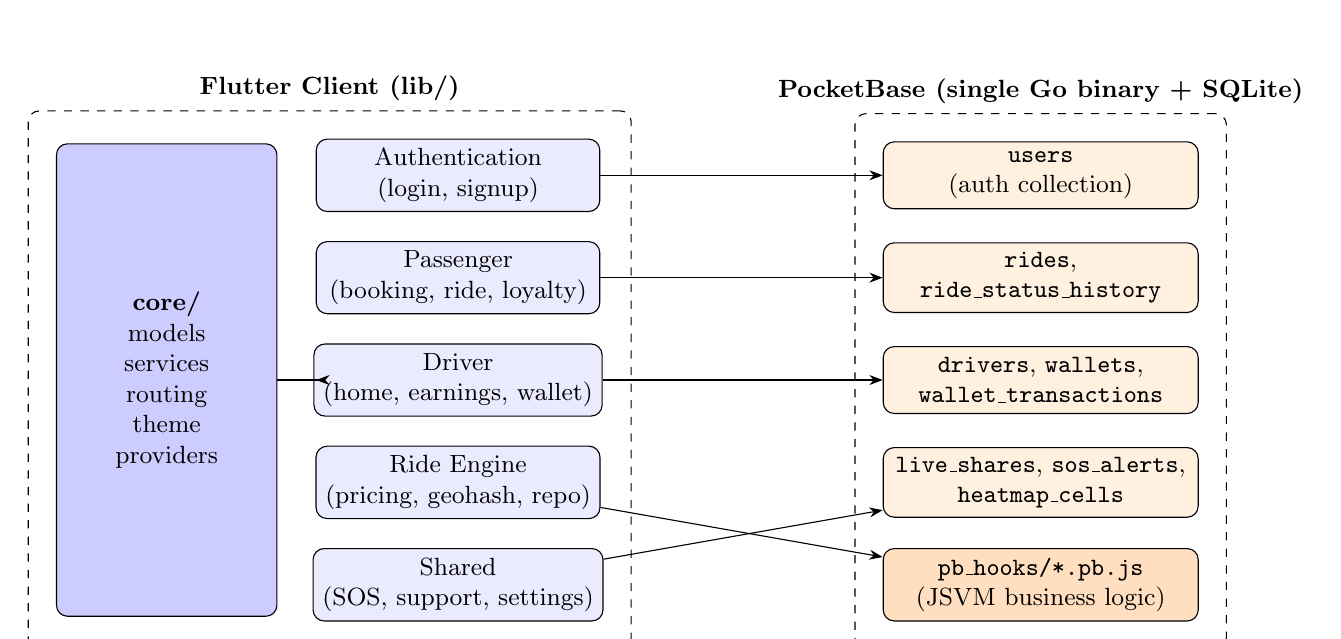
\begin{tikzpicture}[
  every node/.style={font=\small},
  box/.style={draw, rounded corners, fill=blue!8, minimum width=3.6cm, minimum height=0.85cm, align=center},
  pbbox/.style={draw, rounded corners, fill=orange!12, minimum width=4.0cm, minimum height=0.85cm, align=center},
  >=Stealth
]
\node[box] (auth) at (0,5.4) {Authentication\\(login, signup)};
\node[box] (passenger) at (0,4.1) {Passenger\\(booking, ride, loyalty)};
\node[box] (driver) at (0,2.8) {Driver\\(home, earnings, wallet)};
\node[box] (rideengine) at (0,1.5) {Ride Engine\\(pricing, geohash, repo)};
\node[box] (shared) at (0,0.2) {Shared\\(SOS, support, settings)};

\node[box, fill=blue!20, minimum height=6.0cm, minimum width=2.8cm] (core) at (-3.7,2.8) {\textbf{core/}\\models\\services\\routing\\theme\\providers};

\node[pbbox] (userscol) at (7.4,5.4) {\texttt{users}\\(auth collection)};
\node[pbbox] (ridescol) at (7.4,4.1) {\texttt{rides},\\\texttt{ride\_status\_history}};
\node[pbbox] (driverscol) at (7.4,2.8) {\texttt{drivers}, \texttt{wallets},\\\texttt{wallet\_transactions}};
\node[pbbox] (othercol) at (7.4,1.5) {\texttt{live\_shares}, \texttt{sos\_alerts},\\\texttt{heatmap\_cells}};
\node[pbbox, fill=orange!25] (hooks) at (7.4,0.2) {\texttt{pb\_hooks/*.pb.js}\\(JSVM business logic)};

\draw[->] (auth) -- (userscol);
\draw[->] (passenger) -- (ridescol);
\draw[->] (driver) -- (driverscol);
\draw[->] (rideengine) -- (hooks);
\draw[->] (shared) -- (othercol);
\draw[->] (core.east) -- ++(0.5,0) |- (-1.8,2.8);

\node[draw, dashed, rounded corners, fit={(userscol)(ridescol)(driverscol)(othercol)(hooks)}, inner sep=10pt, label={[font=\small\bfseries]above:PocketBase (single Go binary + SQLite)}] {};
\node[draw, dashed, rounded corners, fit={(auth)(passenger)(driver)(rideengine)(shared)(core)}, inner sep=10pt, label={[font=\small\bfseries]above:Flutter Client (lib/)}] {};
\end{tikzpicture}
\caption{High-level architecture: feature-first Flutter modules communicate
with PocketBase collections directly (CRUD + realtime subscriptions) for
non-sensitive reads/writes, and through custom \texttt{pb\_hooks} routes for
every authoritative, financially sensitive mutation.}
\label{fig:architecture}
\end{figure}

\subsection{Technology Stack}

\begin{table}[htbp]
\centering
\caption{Technology stack summary}
\label{tab:stack}
\begin{tabular}{@{}p{3.6cm}p{9.5cm}@{}}
\toprule
\textbf{Layer} & \textbf{Technology} \\
\midrule
Client framework & Flutter 3.43 (beta channel), Dart SDK $\geq$ 3.3.0 \\
State management & \texttt{flutter\_riverpod} 2.6.1 (StreamProvider-based realtime state) \\
Navigation & \texttt{go\_router} 14.3.0 \\
Backend & PocketBase 0.23.x (server), \texttt{pocketbase} Dart SDK 0.24.0 (client) \\
Database & Embedded SQLite (managed entirely by PocketBase) \\
Realtime transport & Server-Sent Events (SSE) via PocketBase \texttt{subscribe()} \\
Local persistence & \texttt{shared\_preferences} (auth token), \texttt{hive}/\texttt{hive\_flutter} (offline cache) \\
Maps \& location & \texttt{google\_maps\_flutter}, \texttt{geolocator}, \texttt{geocoding}, \texttt{flutter\_polyline\_points} \\
Backend hosting & Docker (Alpine multi-stage build), Fly.io (Firecracker micro-VMs) \\
Build target & Android release APK (\texttt{flutter build apk --release}) \\
\bottomrule
\end{tabular}
\end{table}

\subsection{Data Model and Schema Design}
\label{sec:schema}

PocketBase organizes data into \textit{collections}, each backed by a SQLite
table with a JSON-schema-like field definition, optional relation fields,
file fields, and per-operation API rules (\texttt{list}, \texttt{view},
\texttt{create}, \texttt{update}, \texttt{delete}) evaluated server-side. The
MICHWAR schema consists of nine collections, defined declaratively in
\texttt{pocketbase/pb\_migrations/*.js} and applied automatically the first
time the server starts. Table~\ref{tab:collections} summarizes the
collections and their write ownership: \textit{Client} fields are written
directly by the Flutter app subject to API rules; \textit{Hook} fields are
written exclusively by \texttt{pb\_hooks} routes running with full
(\texttt{\$app}) privileges, with \texttt{update}/\texttt{delete} API rules set to
\texttt{null} so that ordinary authenticated requests cannot bypass the
business logic.

\begin{table}[htbp]
\centering
\caption{PocketBase collections and their roles}
\label{tab:collections}
\begin{tabular}{@{}p{3.0cm}p{9.5cm}@{}}
\toprule
\textbf{Collection} & \textbf{Purpose / key fields} \\
\midrule
\texttt{users} (auth) & Email/password auth collection. Profile fields:
\texttt{fullName}, \texttt{phoneNumber}, \texttt{role} (\texttt{passenger}/
\texttt{driver}/\texttt{admin}), \texttt{avatar}, \texttt{loyaltyPoints},
\texttt{loyaltyTier}, \texttt{totalRidesCompleted}, \texttt{savedPlaces},
\texttt{sosContacts}, \texttt{fcmTokens}. \\
\texttt{drivers} & 1:1 relation to \texttt{users}. Vehicle info, verification
status/documents, commission tier/rate, ratings, online/on-trip flags,
live location + geohash, wallet balance. \\
\texttt{rides} & Core ride record: \texttt{passenger}/\texttt{driver} relations,
\texttt{status} (state machine, see \S\ref{sec:ride-lifecycle}),
\texttt{pickup}/\texttt{dropoff} JSON, \texttt{pickupGeohash},
\texttt{candidateDriverIds}, \texttt{fare} JSON (authoritative), \texttt{rating},
live-share token, full timestamp trail. \\
\texttt{ride\_status\_history} & Append-only audit log: one row per status
transition, with the acting user. \\
\texttt{wallets} & 1:1 relation to driver; current balance and low-balance
flag. \\
\texttt{wallet\_transactions} & Immutable ledger of every wallet movement
(ride earnings, top-ups), with the full fare breakdown. \\
\texttt{live\_shares} & Short-lived (6h) publicly readable tokens for live
trip tracking. \\
\texttt{sos\_alerts} & Emergency alerts with ride context and reporter
location/contacts. \\
\texttt{heatmap\_cells} & Aggregated demand counters keyed by a coarse
geohash, incremented atomically. \\
\bottomrule
\end{tabular}
\end{table}

\subsection{Migration Methodology: Firebase to PocketBase}
\label{sec:migration}

The migration was carried out as a systematic, document-by-document mapping
from the Firestore data model and Cloud Functions to the PocketBase
equivalent, recorded in \texttt{pocketbase/MIGRATION\_PLAN.md} and summarized
in Table~\ref{tab:migration}.

\begin{table}[htbp]
\centering
\caption{Firebase $\rightarrow$ PocketBase mapping (excerpt)}
\label{tab:migration}
\begin{tabular}{@{}p{4.3cm}p{4.0cm}p{4.2cm}@{}}
\toprule
\textbf{Firebase construct} & \textbf{PocketBase equivalent} & \textbf{Notes} \\
\midrule
Firebase Auth (phone OTP) & \texttt{users} auth collection (email + password) & \texttt{phoneNumber} becomes a plain profile field \\
\code{users/\{uid\}} (Firestore) & \texttt{users} record & Same id reused as record id \\
\code{drivers/\{uid\}} & \texttt{drivers} (relation \texttt{user}) & 1:1 relation instead of shared document id \\
\code{rides/\{id\}} & \texttt{rides} & \texttt{passengerId}/\texttt{driverId} strings become relation fields \\
\code{rides/\{id\}/status\_history} & \texttt{ride\_status\_history} & relation \texttt{ride} + \texttt{actor} \\
\code{wallets/\{driverId\}} & \texttt{wallets} (relation \texttt{driver}) & 1:1 relation \\
Cloud Storage driver docs & \texttt{drivers.documents} (multi-file field) & + \texttt{documentsMeta} JSON for review status \\
\texttt{onRideRequestCreated} trigger & \texttt{onRecordAfterCreateSuccess} hook on \texttt{rides} & Geohash driver matching \\
\texttt{acceptRide} callable & \texttt{POST /api/michwar/rides/:id/accept} & \\
\texttt{updateRideStatus} callable & \texttt{POST /api/michwar/rides/:id/status} & \\
\texttt{completeRide} callable & \texttt{POST /api/michwar/rides/:id/complete} & Authoritative fare split \\
\texttt{submitRating} callable & \texttt{POST /api/michwar/rides/:id/rate} & \\
\texttt{generateLiveShareLink} callable & \texttt{POST /api/michwar/rides/:id/share} & \\
\bottomrule
\end{tabular}
\end{table}

A representative migration script is shown in
Listing~\ref{lst:migration-users}, which defines the \texttt{users} auth
collection. Each migration file exports an \textit{up} function (applied on
first boot, or when the migration has not yet run) and a \textit{down}
function (used for rollback). One subtlety --- discovered during deployment
and discussed in \S\ref{sec:results-issues} --- is that PocketBase $\geq$
0.23 \textbf{auto-creates a default \texttt{users} auth collection} on a fresh
database, so the migration must first remove that bootstrap collection
before creating the application's own \texttt{users} collection with its
custom fields and API rules.

\begin{lstlisting}[language=JSPB,caption={\texttt{pb\_migrations/1700000001\_users.js} --- defines the \texttt{users} auth collection (with the bootstrap-collection guard added during deployment debugging).},label={lst:migration-users}]
/// <reference path="../pb_data/types.d.ts" />
migrate((app) => {
  // PocketBase >= 0.23 bootstraps a default "users" auth collection on a
  // fresh instance, which collides with the one this migration creates
  // ("Collection name must be unique (case insensitive)"). Since this is
  // the very first migration (runs before anything references "users"),
  // it's safe to drop the bootstrap collection and replace it with ours.
  try {
    const existing = app.findCollectionByNameOrId("users");
    if (existing) {
      app.delete(existing);
    }
  } catch (e) {
    // no existing "users" collection -- nothing to remove
  }

  const collection = new Collection({
    "name": "users",
    "type": "auth",
    "fields": [
      { "name": "fullName", "type": "text", "required": true, "max": 120 },
      { "name": "phoneNumber", "type": "text", "required": true, "max": 20 },
      { "name": "role", "type": "select", "required": true, "maxSelect": 1,
        "values": ["passenger", "driver", "admin"] },
      { "name": "roleSelected", "type": "bool" },
      { "name": "avatar", "type": "file", "maxSelect": 1, "maxSize": 5242880,
        "mimeTypes": ["image/png", "image/jpeg", "image/webp"] },
      { "name": "loyaltyPoints", "type": "number" },
      { "name": "loyaltyTier", "type": "select", "maxSelect": 1,
        "values": ["standard", "eco", "premium"] },
      { "name": "totalRidesCompleted", "type": "number" },
      { "name": "savedPlaces", "type": "json", "maxSize": 200000 },
      { "name": "sosContacts", "type": "json", "maxSize": 200000 },
      { "name": "fcmTokens", "type": "json", "maxSize": 50000 }
    ],
    "passwordAuth": { "enabled": true, "identityFields": ["email"] },
    "listRule": null,
    "viewRule": "id = @request.auth.id || @request.auth.role = 'admin'",
    "createRule": "",
    "updateRule": "id = @request.auth.id",
    "deleteRule": null
  });

  return app.save(collection);
}, (app) => {
  const collection = app.findCollectionByNameOrId("users");
  return app.delete(collection);
});
\end{lstlisting}

\subsection{Backend Business Logic (\texttt{pb\_hooks})}
\label{sec:hooks}

All authoritative, money-affecting, or matching-related logic lives in
\texttt{pocketbase/pb\_hooks/*.pb.js}, loaded automatically by
\texttt{pocketbase serve} into a single shared JavaScript runtime (files are
loaded in filename order, hence the numeric prefixes). This section
describes the three most important hook subsystems: shared constants and
pricing (\S\ref{sec:pricing}), geohash-based driver matching
(\S\ref{sec:geohash}), and the ride lifecycle state machine
(\S\ref{sec:ride-lifecycle}).

\subsubsection{Shared Constants and the Pricing Engine}
\label{sec:pricing}

\texttt{00\_constants.pb.js} defines a single global object, \texttt{MICHWAR},
holding every business constant (commission rates, surcharge bounds, wallet
thresholds, loyalty thresholds, fare formula coefficients, geohash
precision, etc.). This object mirrors --- and must stay in sync with ---
\texttt{lib/core/constants/app\_constants.dart} on the client, which uses the
same constants \textit{only} to show fare \textit{estimates} before a ride
is requested.

\texttt{02\_pricing.pb.js} (Listing~\ref{lst:pricing}) implements the actual
billing formulas. \texttt{mwComputeBaseFare} computes the base fare from the
\textit{actual} GPS-tracked distance and duration of a completed trip,
applies a ride-tier multiplier (\texttt{standard} $\times 1.0$, \texttt{eco}
$\times 0.92$, \texttt{premium} $\times 1.35$), enforces a minimum fare, and
rounds to the nearest 5\,DZD. \texttt{mwComputeSurcharge} derives a small
(1--4\,DZD) platform surcharge deterministically from the ride id, so
repeated calls for the same ride are stable but different rides vary.
\texttt{mwComputeFareBreakdown} then splits the base fare between the driver
and the company according to the driver's current \textbf{commission tier}.

\begin{lstlisting}[language=JSPB,caption={\texttt{pb\_hooks/02\_pricing.pb.js} --- the sole source of billed fare, commission, and loyalty numbers (abridged).},label={lst:pricing}]
function mwRoundToNearest(value, nearest) {
  return Math.round(value / nearest) * nearest;
}

/** Computes the BASE FARE from actual trip distance/duration. */
function mwComputeBaseFare(distanceKm, durationMin, rideTier) {
  var multiplier = MICHWAR.RIDE_TIER_MULTIPLIERS[rideTier];
  if (multiplier == null) multiplier = 1.0;

  var raw =
    MICHWAR.BASE_FARE_FLAG_DZD +
    distanceKm * MICHWAR.FARE_PER_KM_DZD +
    durationMin * MICHWAR.FARE_PER_MINUTE_DZD;

  var tiered = raw * multiplier;

  return tiered < MICHWAR.MINIMUM_FARE_DZD
    ? MICHWAR.MINIMUM_FARE_DZD
    : mwRoundToNearest(tiered, 5);
}

/** Deterministic-but-varying platform surcharge in [MIN, MAX] DZD. */
function mwComputeSurcharge(rideId) {
  var hash = 0;
  for (var i = 0; i < rideId.length; i++) {
    hash = (hash * 31 + rideId.charCodeAt(i)) >>> 0;
  }
  var range = MICHWAR.SURCHARGE_MAX_DZD - MICHWAR.SURCHARGE_MIN_DZD + 1;
  return MICHWAR.SURCHARGE_MIN_DZD + (hash % range);
}

/** Splits the base fare between driver and company, adds the surcharge. */
function mwComputeFareBreakdown(baseFare, surchargeDzd, commissionRate) {
  var commissionAmount = mwRoundToNearest(baseFare * commissionRate, 1);
  var driverPayout = baseFare - commissionAmount;
  var companyRevenue = commissionAmount + surchargeDzd;
  var totalFare = baseFare + surchargeDzd;

  return {
    baseFare: baseFare, surchargeDzd: surchargeDzd, totalFare: totalFare,
    commissionRate: commissionRate, commissionAmount: commissionAmount,
    driverPayout: driverPayout, companyRevenue: companyRevenue,
  };
}

/** Resolves a driver's commission tier from lifetime stats (one-way). */
function mwResolveCommissionTier(ridesCompleted, ratingAverage, currentTier) {
  var alreadyElite = currentTier === "tier2";
  var qualifiesForElite =
    ridesCompleted >= MICHWAR.ELITE_MIN_COMPLETED_RIDES &&
    ratingAverage >= MICHWAR.ELITE_MIN_AVERAGE_RATING;

  if (alreadyElite || qualifiesForElite) {
    return { tier: "tier2", commissionRate: MICHWAR.TIER2_COMMISSION_RATE,
             driverShareRate: MICHWAR.TIER2_DRIVER_RATE };
  }
  return { tier: "tier1", commissionRate: MICHWAR.TIER1_COMMISSION_RATE,
           driverShareRate: MICHWAR.TIER1_DRIVER_RATE };
}
\end{lstlisting}

Two driver commission tiers exist: \textbf{Tier 1 (Base)}, where the company
retains 15\% of the base fare and the driver keeps 85\%, and \textbf{Tier 2
(Elite)}, where the company retains only 7\% and the driver keeps 93\%.
Promotion to Elite requires at least 100 completed rides \textit{and} an
average rating of at least 4.0, and --- once granted --- is never revoked
even if the average later dips (a one-way ratchet, implemented by the
\texttt{alreadyElite} check). Figure~\ref{fig:commission} visualizes this
split. The platform surcharge (1--4\,DZD) is 100\% company revenue and is
\textit{not} part of the commission base.

\begin{figure}[htbp]
\centering
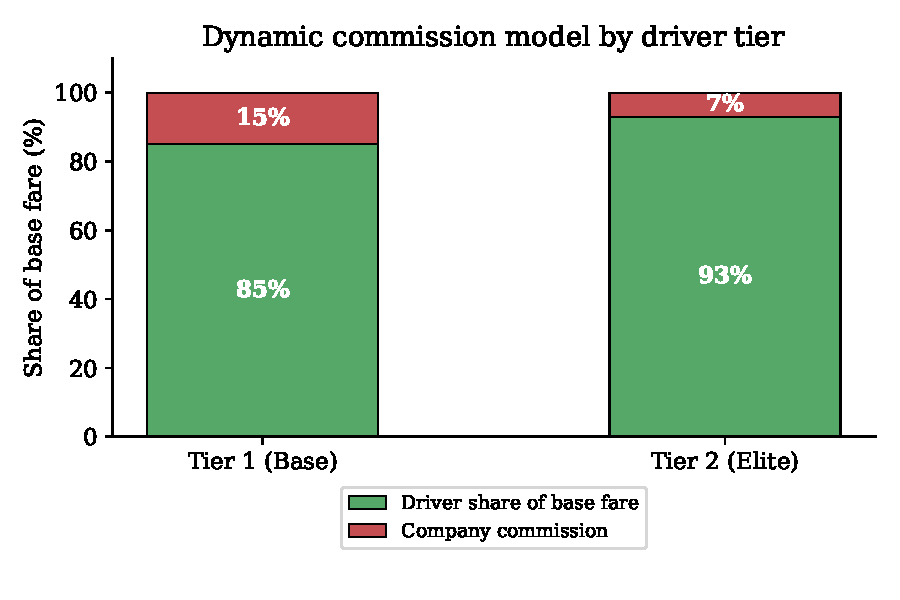
\includegraphics[width=0.62\textwidth]{commission_tiers}
\caption{Dynamic commission model: the driver's share of the base fare
increases from 85\% to 93\% upon promotion to the Elite (Tier~2) tier,
which requires $\geq$100 completed rides and an average rating $\geq$4.0.}
\label{fig:commission}
\end{figure}

\textbf{MICHWAR Points} (the loyalty currency) are awarded on every
completed ride as $\lfloor \text{totalFare} / 100 \rfloor \times 2$. A
passenger reaches the \textit{eco} tier (5\% discount on estimates) at 50
points and the \textit{premium} tier (access to premium-tier rides) at 200
points, via \texttt{mwResolveLoyaltyTier}.

\subsubsection{Geohash-Based Driver Matching}
\label{sec:geohash}

MICHWAR has no native geospatial index (PocketBase/SQLite has no built-in
geo type), so proximity matching is implemented with \textbf{geohashing}:
each driver's location is encoded into a base-32 geohash string
(\texttt{locationGeohash}, precision 7, $\approx 153\,\text{m} \times
153\,\text{m}$ cells) and stored as an indexed text field. The \textit{same}
geohash algorithm is implemented twice --- once in Dart
(\texttt{lib/core/utils/geohash\_util.dart}, used for client-side estimates and
the driver's periodic location pings) and once in JavaScript
(\texttt{pb\_hooks/01\_geohash.pb.js}, used server-side for matching) --- to
guarantee that cell boundaries agree between client and server.

When a passenger creates a ride request (\texttt{rides} record with
\texttt{status = "searching"}), an \texttt{onRecordAfterCreateSuccess} hook on
\texttt{rides} runs \texttt{mwMatchDriversForRide}. This function:

\begin{enumerate}[nosep]
  \item Starts at \texttt{DEFAULT\_DRIVER\_SEARCH\_RADIUS\_KM} (3\,km).
  \item Computes the geohash precision whose cell size is $\geq$ the current
    radius, enumerates the neighboring cells covering a circle of that
    radius (\texttt{mwNeighborsForRadius}), and queries \texttt{drivers} where
    \texttt{isOnline = true}, \texttt{isOnTrip = false},
    \texttt{verificationStatus = 'approved'}, \texttt{walletBalance} is above
    the low-balance threshold, and \texttt{locationGeohash} falls within the
    cell-prefix range.
  \item Filters the resulting candidates by true Haversine distance
    (\texttt{mwDistanceKm}) $\leq$ radius.
  \item If no candidates are found, \textbf{doubles the radius} and repeats,
    up to \texttt{MAX\_DRIVER\_SEARCH\_RADIUS\_KM} (10\,km); if still empty,
    sets \texttt{status = "no\_drivers\_found"}.
  \item Otherwise sorts candidates by distance (with a "Heading Home" bonus,
    described below) and writes up to \texttt{MAX\_CANDIDATE\_DRIVERS} (10)
    driver ids into \texttt{rides.candidateDriverIds}, which each driver app
    subscribes to via realtime.
\end{enumerate}

The \textbf{"Heading Home"} feature lets a driver mark a destination they are
driving toward at the end of their shift. If a candidate driver has
\texttt{headingHomeEnabled} and the bearing from their current position to
their home destination (\texttt{mwBearingDeg}) is within
\texttt{headingHomeBearingTolerance} (default $30^{\circ}$) of the bearing to the
ride's drop-off, their \textit{effective} distance is reduced by 1\,km,
making them more likely to be offered a "last ride home" that is convenient
for them. Figure~\ref{fig:geohash} illustrates the expanding-radius search.

\begin{figure}[htbp]
\centering
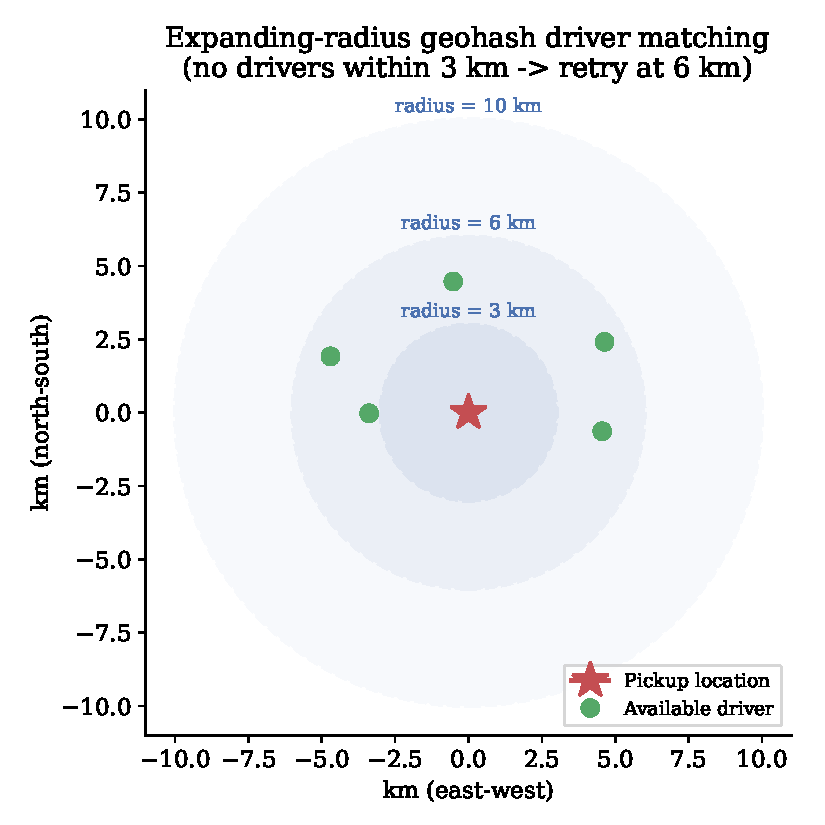
\includegraphics[width=0.62\textwidth]{geohash_matching}
\caption{Expanding-radius geohash matching: the matcher first searches the
3\,km cell neighborhood around the pickup point; if no eligible driver is
found, it doubles the radius (6\,km, then 10\,km) until a candidate is found
or the maximum radius is reached.}
\label{fig:geohash}
\end{figure}

\subsubsection{The Ride Lifecycle State Machine}
\label{sec:ride-lifecycle}

\texttt{rides.status} follows a strict state machine, enforced entirely
server-side. A passenger may only \textit{create} a ride (which is forced to
\texttt{status = "searching"}); every subsequent transition is performed by one
of the \texttt{pb\_hooks/12\_rides.pb.js} routes running inside
\texttt{\$app.runInTransaction()}, which is PocketBase's equivalent of a
Firestore transaction. Direct client \texttt{update}/\texttt{delete} on
\texttt{rides} is disabled at the API-rule level (\texttt{updateRule: null}), and
an \texttt{onRecordUpdateRequest} hook additionally reverts any of the
protected fields (\texttt{status}, \texttt{driver}, \texttt{fare}, timestamps,
etc.) listed in \texttt{MW\_RIDE\_PROTECTED\_FIELDS} if a non-admin somehow
submits an update. Figure~\ref{fig:statemachine} shows the resulting state
machine.

\begin{figure}[htbp]
\centering
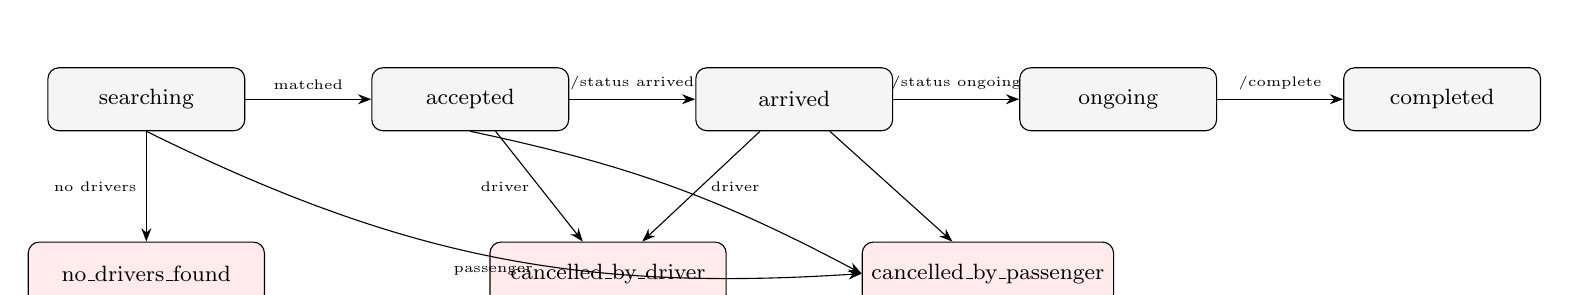
\begin{tikzpicture}[
  every node/.style={font=\footnotesize},
  state/.style={draw, rounded corners, fill=gray!8, minimum width=2.5cm, minimum height=0.8cm, align=center},
  bad/.style={draw, rounded corners, fill=red!8, minimum width=3.0cm, minimum height=0.8cm, align=center},
  >=Stealth, node distance=1.3cm and 1.6cm
]
\node[state] (searching) {searching};
\node[state, right=of searching] (accepted) {accepted};
\node[state, right=of accepted] (arrived) {arrived};
\node[state, right=of arrived] (ongoing) {ongoing};
\node[state, right=of ongoing] (completed) {completed};

\node[bad, below=1.4cm of searching] (nodrivers) {no\_drivers\_found};
\node[bad, below right=1.4cm and -0.4cm of arrived] (cancelpax) {cancelled\_by\_passenger};
\node[bad, below left=1.4cm and -0.4cm of arrived] (canceldriver) {cancelled\_by\_driver};

\draw[->] (searching) -- node[above,font=\tiny]{matched} (accepted);
\draw[->] (searching) -- node[left,font=\tiny]{no drivers} (nodrivers);
\draw[->] (accepted) -- node[above,font=\tiny]{/status arrived} (arrived);
\draw[->] (arrived) -- node[above,font=\tiny]{/status ongoing} (ongoing);
\draw[->] (ongoing) -- node[above,font=\tiny]{/complete} (completed);
\draw[->] (accepted) -- node[left,font=\tiny]{driver} (canceldriver);
\draw[->] (arrived) -- node[right,font=\tiny]{driver} (canceldriver);
\draw[->] (searching.south) to[bend right=15] node[below,font=\tiny]{passenger} (cancelpax.west);
\draw[->] (accepted.south) to[bend left=8] (cancelpax.west);
\draw[->] (arrived) -- (cancelpax);
\end{tikzpicture}
\caption{Ride lifecycle state machine implemented in
\texttt{pb\_hooks/12\_rides.pb.js}. All transitions other than the initial
\texttt{create} (passenger $\rightarrow$ \texttt{searching}) are performed
inside a server-side transaction by one of the
\code{/api/michwar/rides/:id/\{accept,status,complete\}} routes.}
\label{fig:statemachine}
\end{figure}

Listing~\ref{lst:accept} shows the \texttt{/accept} route: it atomically
checks that the ride is still \texttt{searching} and unclaimed, that the
requesting driver is not already on a trip and has sufficient wallet
balance, then assigns the driver, flips the ride to \texttt{accepted}, marks
the driver \texttt{isOnTrip = true}, and appends a
\texttt{ride\_status\_history} row --- all inside one transaction so that two
drivers can never simultaneously "win" the same ride.

\begin{lstlisting}[language=JSPB,caption={\texttt{pb\_hooks/12\_rides.pb.js} --- \texttt{POST /api/michwar/rides/:id/accept} (race-safe ride acceptance).},label={lst:accept}]
routerAdd("POST", "/api/michwar/rides/{id}/accept", (e) => {
  if (!e.auth) throw new UnauthorizedError("You must be signed in.");

  var rideId = e.request.pathValue("id");

  $app.runInTransaction((txApp) => {
    var ride = txApp.findRecordById("rides", rideId);
    var driver = txApp.findFirstRecordByFilter(
      "drivers", "user = {:uid}", { uid: e.auth.id });

    if (ride.get("status") !== "searching" || ride.get("driver")) {
      throw new BadRequestError(
        "This ride has already been accepted by another driver.");
    }
    if (driver.get("isOnTrip")) {
      throw new BadRequestError("You already have an active trip.");
    }
    if ((driver.get("walletBalance") || 0)
        <= MICHWAR.WALLET_LOW_BALANCE_THRESHOLD_DZD) {
      throw new BadRequestError(
        "Your wallet balance is too low to accept new rides.");
    }

    ride.set("driver", e.auth.id);
    ride.set("status", "accepted");
    ride.set("acceptedAt", new Date().toISOString());
    txApp.save(ride);

    driver.set("isOnTrip", true);
    txApp.save(driver);

    var history = new Record(txApp.findCollectionByNameOrId("ride_status_history"));
    history.set("ride", rideId);
    history.set("status", "accepted");
    history.set("actor", e.auth.id);
    txApp.save(history);
  });

  return e.json(200, { ok: true });
}, $apis.requireAuth());
\end{lstlisting}

The \texttt{/complete} route (the most complex in the system, $\approx$130
lines) is invoked by the driver when a trip ends, supplying the
GPS-tracked \texttt{actualDistanceKm} and \texttt{actualDurationMin}. Within a
single transaction it: (1) computes the fare breakdown via
\texttt{02\_pricing.pb.js}; (2) debits the driver's wallet by the company's
revenue share and writes the new balance to both \texttt{drivers} and
\texttt{wallets}; (3) appends an immutable \texttt{wallet\_transactions} ledger
row containing the full breakdown; (4) increments the driver's
\texttt{ridesCompleted} and re-evaluates their commission tier; (5) credits
the passenger's loyalty points and re-evaluates their loyalty tier; and (6)
writes the authoritative \texttt{fare} object onto the \texttt{rides} record and
marks it \texttt{completed}. Because every one of these writes happens inside
\texttt{\$app.runInTransaction()}, a crash or error at any point rolls back the
entire set --- there is no possibility of, for example, debiting a driver's
wallet without recording the corresponding ledger entry.

\subsection{Client Architecture: State Management and Realtime Data}
\label{sec:client-state}

The Flutter client uses \textbf{Riverpod} (\texttt{flutter\_riverpod}) for
dependency injection and reactive state. Listing~\ref{lst:providers} shows
an excerpt of \texttt{lib/core/providers/app\_providers.dart}: the
\texttt{pocketbaseProvider} exposes the shared \texttt{PocketBase} client (the
instance is created once in \texttt{main.dart} via
\texttt{PocketBaseService.getInstance()} and provided as an override --- see
Listing~\ref{lst:pbservice}); \texttt{authStateProvider} is a
\texttt{StreamProvider<String?>} derived from
\texttt{AuthService.authStateChanges()}; and \texttt{watchRelatedRecord} is a
generic helper that subscribes to the single record in a collection whose
relation field matches the current user (used for both
\texttt{driverProfileProvider} and \texttt{walletProvider}). Each subscription
immediately emits the current value via \texttt{getFirstListItem}, then again
on every realtime \texttt{create}/\texttt{update}/\texttt{delete} event delivered
over the PocketBase SSE stream --- functionally equivalent to a Firestore
\texttt{DocumentReference.snapshots()} listener, but backed by PocketBase's
realtime API.

\begin{lstlisting}[language=Dart,caption={\texttt{lib/core/providers/app\_providers.dart} --- generic realtime "watch the record related to me" provider helper (abridged).},label={lst:providers}]
final pocketbaseProvider = Provider<PocketBase>((ref) {
  throw UnimplementedError(
    'pocketbaseProvider must be overridden in main.dart with the '
    'PocketBaseService-initialized client.');
});

final authStateProvider = StreamProvider<String?>((ref) {
  return ref.watch(authServiceProvider).authStateChanges();
});

final driverProfileProvider = StreamProvider<DriverModel?>((ref) {
  final uid = ref.watch(authStateProvider).valueOrNull;
  if (uid == null) return Stream.value(null);
  final pb = ref.watch(pocketbaseProvider);
  return watchRelatedRecord(
    pb: pb, collection: PbCollections.drivers, relationField: 'user',
    relationValue: uid, fromMap: DriverModel.fromMap,
  );
});

Stream<T?> watchRelatedRecord<T>({
  required PocketBase pb,
  required String collection,
  required String relationField,
  required String relationValue,
  required T Function(String id, Map<String, dynamic> map) fromMap,
}) {
  final controller = StreamController<T?>();
  UnsubscribeFunc? unsubscribe;

  Future<void> start() async {
    try {
      final record = await pb.collection(collection).getFirstListItem(
        pb.filter('$relationField = {:value}', {'value': relationValue}));
      controller.add(fromMap(record.id, record.toJson()));

      unsubscribe = await pb.collection(collection).subscribe(record.id, (e) {
        if (e.action == 'delete') {
          controller.add(null);
        } else if (e.record != null) {
          controller.add(fromMap(e.record!.id, e.record!.toJson()));
        }
      });
    } catch (_) {
      controller.add(null);
    }
  }

  controller.onListen = () {
    start().catchError((Object error, StackTrace stack) {
      controller.addError(error, stack);
    });
  };
  controller.onCancel = () async {
    await unsubscribe?.call();
    await controller.close();
  };

  return controller.stream;
}
\end{lstlisting}

Listing~\ref{lst:pbservice} shows \texttt{pocketbase\_service.dart}: it
resolves the backend base URL via \texttt{pocketbaseBaseUrl()}, which defaults
to \texttt{http://10.0.2.2:8090} on the Android emulator (the special address
that routes to the host machine's \texttt{localhost}), \texttt{http://127.0.0.1:
8090} elsewhere, and is overridable at build time with
\texttt{--dart-define=POCKETBASE\_URL=...} --- the mechanism used to point
release builds at the public Fly.io deployment (\S\ref{sec:deployment}). The
auth session is persisted across app restarts using an
\texttt{AsyncAuthStore} backed by \texttt{shared\_preferences}, replacing
Firebase Auth's automatic session persistence.

\begin{lstlisting}[language=Dart,caption={\texttt{lib/core/services/pocketbase\_service.dart} --- PocketBase client singleton with persisted auth.},label={lst:pbservice}]
String pocketbaseBaseUrl() {
  const override = String.fromEnvironment('POCKETBASE_URL');
  if (override.isNotEmpty) return override;

  if (kIsWeb) return 'http://127.0.0.1:8090';
  if (Platform.isAndroid) return 'http://10.0.2.2:8090';
  return 'http://127.0.0.1:8090';
}

class PocketBaseService {
  PocketBaseService._(this.pb);
  final PocketBase pb;
  static PocketBaseService? _instance;

  static Future<PocketBaseService> getInstance() async {
    if (_instance != null) return _instance!;

    final prefs = await SharedPreferences.getInstance();
    final store = AsyncAuthStore(
      save: (String data) async => prefs.setString('pb_auth', data),
      initial: prefs.getString('pb_auth'),
      clear: () async => prefs.remove('pb_auth'),
    );

    final pb = PocketBase(pocketbaseBaseUrl(), authStore: store);
    _instance = PocketBaseService._(pb);
    return _instance!;
  }
}
\end{lstlisting}

A notable implementation detail encountered during the build (detailed in
\S\ref{sec:results-issues}) concerns the \texttt{pocketbase} Dart package's
authentication-state stream. Version 0.24.0 exposes
\texttt{AuthStore.onChange} as a \textbf{Dart \texttt{Stream<AuthStoreEvent>}}
(replacing the older callback-based API), and exposes the current user as
\texttt{AuthStore.record} (an \texttt{AuthRecord?}) rather than the older
\texttt{AuthStore.model}. Listing~\ref{lst:authservice} shows the corrected
\texttt{authStateChanges()} implementation, which wraps the SDK's stream in a
\texttt{StreamController} so it can be combined with an immediate "current
value" emission --- mirroring the ergonomics of
\texttt{FirebaseAuth.authStateChanges()}.

\begin{lstlisting}[language=Dart,caption={\texttt{lib/core/services/auth\_service.dart} --- authentication state stream over the PocketBase 0.24.0 \texttt{AuthStore.onChange} stream API.},label={lst:authservice}]
class AuthService {
  AuthService(this._pb);
  final PocketBase _pb;

  bool get isSignedIn => _pb.authStore.isValid;
  String? get currentUserId => _pb.authStore.record?.id;

  /// Emits the current user id immediately, then again on every change;
  /// `null` means "signed out".
  Stream<String?> authStateChanges() {
    final controller = StreamController<String?>();
    controller.add(_pb.authStore.record?.id);

    final subscription = _pb.authStore.onChange.listen((event) {
      controller.add(event.record?.id);
    });

    controller.onCancel = () {
      subscription.cancel();
      controller.close();
    };

    return controller.stream;
  }

  Future<RecordAuth> signUp({
    required String email, required String password,
    required String fullName, required String phoneNumber,
  }) async {
    await _pb.collection(PbCollections.users).create(body: {
      'email': email, 'password': password, 'passwordConfirm': password,
      'fullName': fullName, 'phoneNumber': phoneNumber, 'role': 'passenger',
    });
    return signIn(email: email, password: password);
  }

  Future<RecordAuth> signIn({required String email, required String password}) {
    return _pb.collection(PbCollections.users).authWithPassword(email, password);
  }

  Future<void> signOut() async => _pb.authStore.clear();
}
\end{lstlisting}

\subsection{Build Process: Producing a Release APK}
\label{sec:build}

Although the Flutter source tree (\texttt{lib/}) had been fully migrated, the
project had originally been authored without ever running \texttt{flutter
create}, so the Android (and iOS/web/desktop) platform projects did not
exist. Running \texttt{flutter create .} from the project root scaffolds
\texttt{android/}, \texttt{ios/}, \texttt{web/}, \texttt{windows/}, \texttt{linux/},
and \texttt{macos/} \textit{without} touching the existing \texttt{lib/} source
--- a safe, additive operation. After \texttt{flutter pub get}, the release
APK is produced with:

\begin{lstlisting}[language=bash,caption={Release APK build command, with the PocketBase backend URL baked in as a compile-time constant.}]
flutter build apk --release \
  --dart-define=POCKETBASE_URL=https://michwar-pb.fly.dev
\end{lstlisting}

\texttt{--dart-define} injects a compile-time environment constant that
\texttt{pocketbaseBaseUrl()} (Listing~\ref{lst:pbservice}) reads via
\texttt{String.fromEnvironment('POCKETBASE\_URL')} --- this is how the same
codebase produces a build that talks to \texttt{10.0.2.2:8090} (emulator), a
LAN IP (local testing on a physical device), or the public Fly.io URL
(distributable release), with no source changes.

\subsection{Deployment Methodology: Containerization and Fly.io}
\label{sec:deployment}

For the distributed APK to "just work" for any user on any network, the
PocketBase backend must be reachable over the public internet with HTTPS
--- a LAN IP (e.g.\ \texttt{192.168.1.50:8090}) only works for devices on the
same Wi-Fi as the development machine. The backend was therefore
containerized and deployed to \textbf{Fly.io}, which offers a free-tier
allowance of shared-CPU micro-VMs (Firecracker) with persistent volumes and
automatic HTTPS on a \texttt{*.fly.dev} subdomain.

Listing~\ref{lst:dockerfile} shows the multi-stage \texttt{Dockerfile}: the
\texttt{builder} stage (Alpine) downloads the official PocketBase v0.23.12
release binary for \texttt{linux\_amd64} and unzips it; the final stage copies
only the binary plus \texttt{pb\_migrations/} and \texttt{pb\_hooks/} into a
minimal Alpine image, exposes port 8090, and declares \texttt{/pb/pb\_data} as
a volume mount point for the SQLite database and uploaded files. The
resulting image is only \textbf{18\,MB}.

\begin{lstlisting}[language=bash,caption={\texttt{pocketbase/Dockerfile} --- multi-stage build producing an 18\,MB PocketBase image.},label={lst:dockerfile}]
# --- Stage 1: fetch the PocketBase binary -----------------------------
FROM alpine:3.20 AS builder
ARG PB_VERSION=0.23.12

RUN apk add --no-cache unzip curl ca-certificates \
    && curl -fsSL "https://github.com/pocketbase/pocketbase/releases/download/v${PB_VERSION}/pocketbase_${PB_VERSION}_linux_amd64.zip" -o /tmp/pb.zip \
    && unzip /tmp/pb.zip -d /pb \
    && rm /tmp/pb.zip

# --- Stage 2: minimal runtime image ------------------------------------
FROM alpine:3.20
RUN apk add --no-cache ca-certificates
WORKDIR /pb

COPY --from=builder /pb/pocketbase /pb/pocketbase
COPY pb_migrations ./pb_migrations
COPY pb_hooks ./pb_hooks

VOLUME /pb/pb_data
EXPOSE 8090
CMD ["/pb/pocketbase", "serve", "--http=0.0.0.0:8090"]
\end{lstlisting}

Listing~\ref{lst:flytoml} shows the generated \texttt{fly.toml}: a 1\,GB
persistent volume \texttt{pb\_data} is mounted at \texttt{/pb/pb\_data} (matching
the Dockerfile's \texttt{VOLUME}), \texttt{force\_https = true} provides
automatic TLS termination, and \texttt{min\_machines\_running = 1} keeps the
instance always-on (avoiding cold-start latency and keeping SSE realtime
subscriptions connected), at the cost of consuming part of the free-tier
shared-CPU allowance.

\begin{lstlisting}[language=bash,caption={\texttt{pocketbase/fly.toml} --- Fly.io application configuration.},label={lst:flytoml}]
app = 'michwar-pb'
primary_region = 'cdg'

[build]

[[mounts]]
  source = 'pb_data'
  destination = '/pb/pb_data'

[http_service]
  internal_port = 8090
  force_https = true
  auto_stop_machines = 'off'
  auto_start_machines = true
  min_machines_running = 1

[[vm]]
  size = 'shared-cpu-1x'
  memory = '256mb'
\end{lstlisting}

Figure~\ref{fig:pipeline} summarizes the end-to-end deployment pipeline,
from source to a publicly reachable HTTPS endpoint.

\begin{figure}[htbp]
\centering
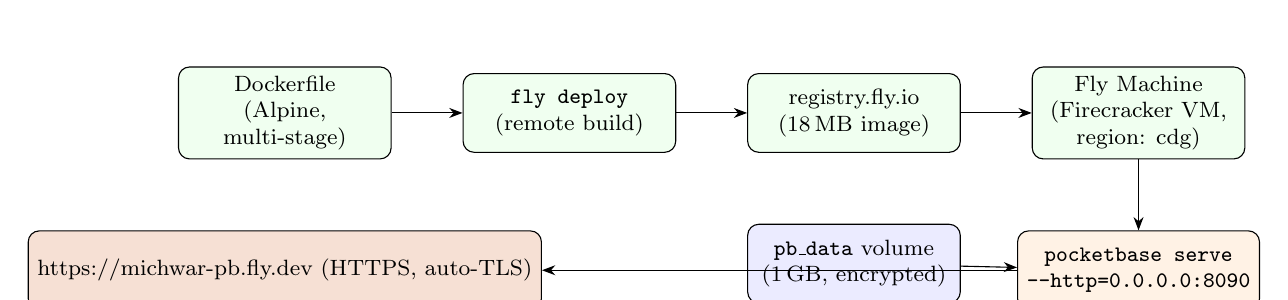
\begin{tikzpicture}[
  every node/.style={font=\footnotesize},
  block/.style={draw, rounded corners, fill=green!6, minimum width=2.7cm, minimum height=1.0cm, align=center},
  >=Stealth, node distance=0.9cm and 0.9cm
]
\node[block] (df) {Dockerfile\\(Alpine,\\multi-stage)};
\node[block, right=of df] (build) {\texttt{fly deploy}\\(remote build)};
\node[block, right=of build] (registry) {registry.fly.io\\(18\,MB image)};
\node[block, right=of registry] (machine) {Fly Machine\\(Firecracker VM,\\region: cdg)};
\node[block, fill=orange!10, below=of machine] (pb) {\texttt{pocketbase serve}\\\texttt{--http=0.0.0.0:8090}};
\node[block, fill=blue!8, below=of registry] (vol) {\texttt{pb\_data} volume\\(1\,GB, encrypted)};
\node[block, fill=michwarorange!25, below=of df, minimum width=5.6cm] (url) {\url{https://michwar-pb.fly.dev} (HTTPS, auto-TLS)};

\draw[->] (df) -- (build);
\draw[->] (build) -- (registry);
\draw[->] (registry) -- (machine);
\draw[->] (machine) -- (pb);
\draw[->] (vol) -- (pb);
\draw[->] (pb.west) -- (url.east);
\end{tikzpicture}
\caption{Deployment pipeline: a multi-stage Docker build is sent to Fly.io's
remote builder, pushed to \texttt{registry.fly.io}, and run as a Firecracker
micro-VM with a persistent volume for \texttt{pb\_data}, exposed publicly over
HTTPS.}
\label{fig:pipeline}
\end{figure}


% ===========================================================================
\section{Results}
\label{sec:results}
% ===========================================================================

\subsection{Codebase Composition}

Table~\ref{tab:loc} and Figure~\ref{fig:loc} summarize the size of the
resulting codebase by module, measured in lines of code. The Flutter client
(\texttt{lib/}) totals approximately 8{,}169 lines across \texttt{core/} and the
five feature modules, while the PocketBase backend (\texttt{pb\_hooks/} and
\texttt{pb\_migrations/}) totals 1{,}374 lines --- a useful illustration of how
much server-side logic a self-hosted backend requires relative to a
"backend-less" Firebase setup, where most of this logic would otherwise live
in Cloud Functions written in TypeScript.

\begin{table}[htbp]
\centering
\caption{Lines of code by module}
\label{tab:loc}
\begin{tabular}{@{}lr@{}}
\toprule
\textbf{Module} & \textbf{Lines of code} \\
\midrule
\texttt{lib/core/} (models, services, routing, theme, providers) & 2{,}444 \\
\texttt{lib/features/authentication/} & 845 \\
\texttt{lib/features/passenger/} & 1{,}768 \\
\texttt{lib/features/driver/} & 1{,}659 \\
\texttt{lib/features/ride\_engine/} & 717 \\
\texttt{lib/features/shared/} & 736 \\
\midrule
\textbf{Flutter client total} & \textbf{8{,}169} \\
\midrule
\texttt{pocketbase/pb\_hooks/} (business logic) & 1{,}059 \\
\texttt{pocketbase/pb\_migrations/} (schema) & 315 \\
\midrule
\textbf{PocketBase backend total} & \textbf{1{,}374} \\
\bottomrule
\end{tabular}
\end{table}

\begin{figure}[htbp]
\centering
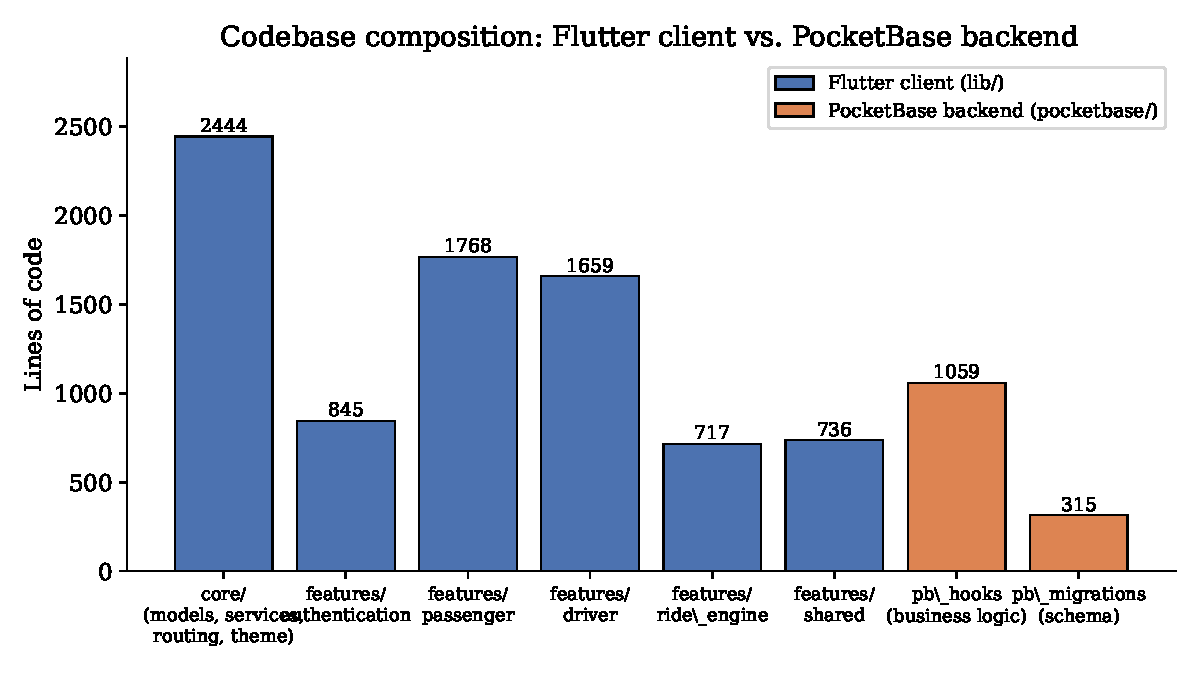
\includegraphics[width=0.85\textwidth]{codebase_composition}
\caption{Lines of code per module. The Flutter client (blue) is roughly six
times larger than the PocketBase backend (orange), reflecting that the
backend logic is concentrated in nine compact hook files plus declarative
schema migrations.}
\label{fig:loc}
\end{figure}

\subsection{Build Results}

The release Android APK built successfully with \texttt{flutter build apk
--release}, producing \texttt{build/app/outputs/flutter-apk/app-release.apk}
at approximately \textbf{54\,MB} (56{,}613{,}947 bytes). The build environment
was Flutter 3.43.0 (beta channel) with Android SDK 36.1.0 on Windows. The
only diagnostics emitted were harmless Java~8 source/target deprecation
warnings from the Android Gradle plugin and standard font-asset
tree-shaking notices (e.g.\ \texttt{MaterialIcons-Regular.otf} reduced by
99.4\%). No application code changes were required beyond the dependency and
API-version fixes described in \S\ref{sec:results-issues}.

\subsection{Deployment Outcome}

The containerized PocketBase backend was deployed to Fly.io under the
application name \texttt{michwar-pb} in the \texttt{cdg} (Paris) region. The
final, successful deploy produced:

\begin{itemize}[nosep]
  \item A Docker image of \textbf{18\,MB} pushed to
    \texttt{registry.fly.io/michwar-pb}.
  \item A dedicated IPv6 and a shared IPv4 address, with automatic HTTPS via
    Fly's edge proxy.
  \item A running Firecracker machine with a 1\,GB encrypted persistent
    volume mounted at \texttt{/pb/pb\_data}.
  \item A publicly reachable endpoint at
    \textbf{\url{https://michwar-pb.fly.dev}}, with the PocketBase Admin UI
    at \texttt{/\_/} and the REST/realtime API at \texttt{/api/}.
\end{itemize}

\texttt{fly status} confirmed the machine state as \texttt{started}, and
\texttt{fly logs} showed PocketBase applying all nine schema migrations
successfully on first boot and beginning to serve HTTP traffic. The release
APK was then rebuilt with
\texttt{--dart-define=POCKETBASE\_URL=https://michwar-pb.fly.dev}
(\S\ref{sec:build}), producing a final distributable artifact that requires
no configuration on the end user's device or network.

\subsection{Worked Example: Fare and Commission Computation}

To validate the pricing engine described in \S\ref{sec:pricing}, consider a
completed \texttt{standard}-tier ride of 8.4\,km over 22\,minutes, completed by
a Tier-1 (Base) driver:

\begin{align}
\text{raw} &= 100 + (8.4 \times 35) + (22 \times 5) = 100 + 294 + 110 = 504 \\
\text{tiered} &= 504 \times 1.0 = 504 \\
\text{baseFare} &= \max(150,\ \text{round}_5(504)) = 505 \\
\text{surcharge} &= 3 \quad (\text{deterministic, } \in [1,4]) \\
\text{commission} &= \text{round}_1(505 \times 0.15) = 76 \\
\text{driverPayout} &= 505 - 76 = 429 \\
\text{companyRevenue} &= 76 + 3 = 79 \\
\text{totalFare} &= 505 + 3 = 508 \\
\text{pointsAwarded} &= \lfloor 508/100 \rfloor \times 2 = 10
\end{align}

Figure~\ref{fig:fare} visualizes the resulting split of the 508\,DZD total
fare. This is the exact computation performed inside
\texttt{POST /api/michwar/rides/:id/complete}; the breakdown is persisted both
on \texttt{rides.fare} and as a \texttt{wallet\_transactions} ledger row.

\begin{figure}[htbp]
\centering
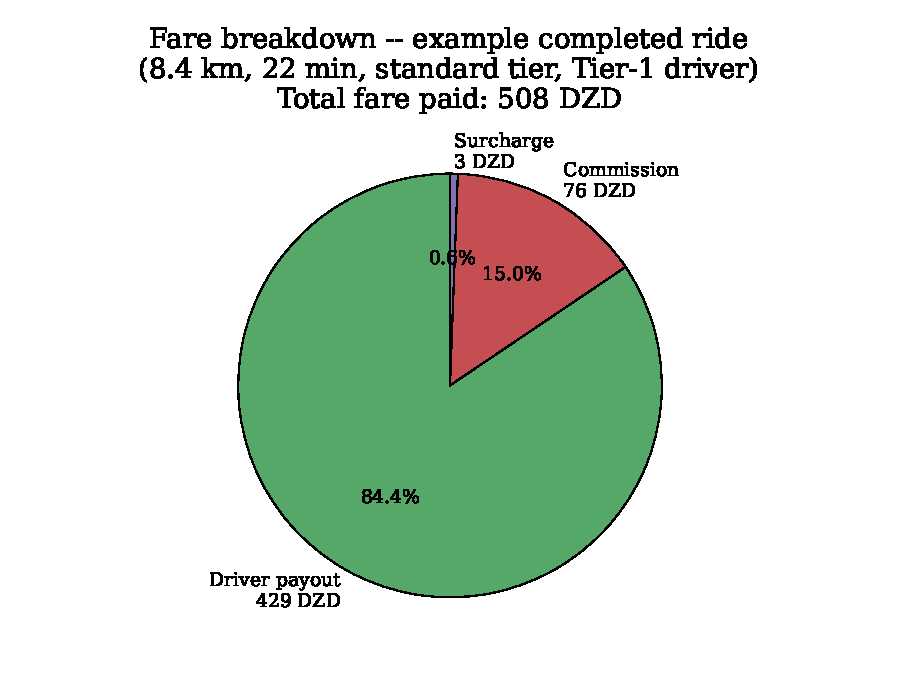
\includegraphics[width=0.6\textwidth]{fare_breakdown}
\caption{Worked example: fare breakdown for an 8.4\,km / 22\,min standard-tier
ride completed by a Tier-1 driver. The driver receives 429\,DZD (84.4\%), the
company receives 79\,DZD in commission + surcharge (15.6\%), for a total
fare of 508\,DZD.}
\label{fig:fare}
\end{figure}

\subsection{Issues Encountered and Resolutions}
\label{sec:results-issues}

The path from a migrated source tree to a live, publicly reachable backend
surfaced a sequence of distinct issues spanning the Flutter toolchain, the
Windows shell, a backend SDK version mismatch, and the PocketBase server
itself. Figure~\ref{fig:timeline} and Table~\ref{tab:issues} summarize them
chronologically; each is discussed in turn below.

\begin{figure}[htbp]
\centering
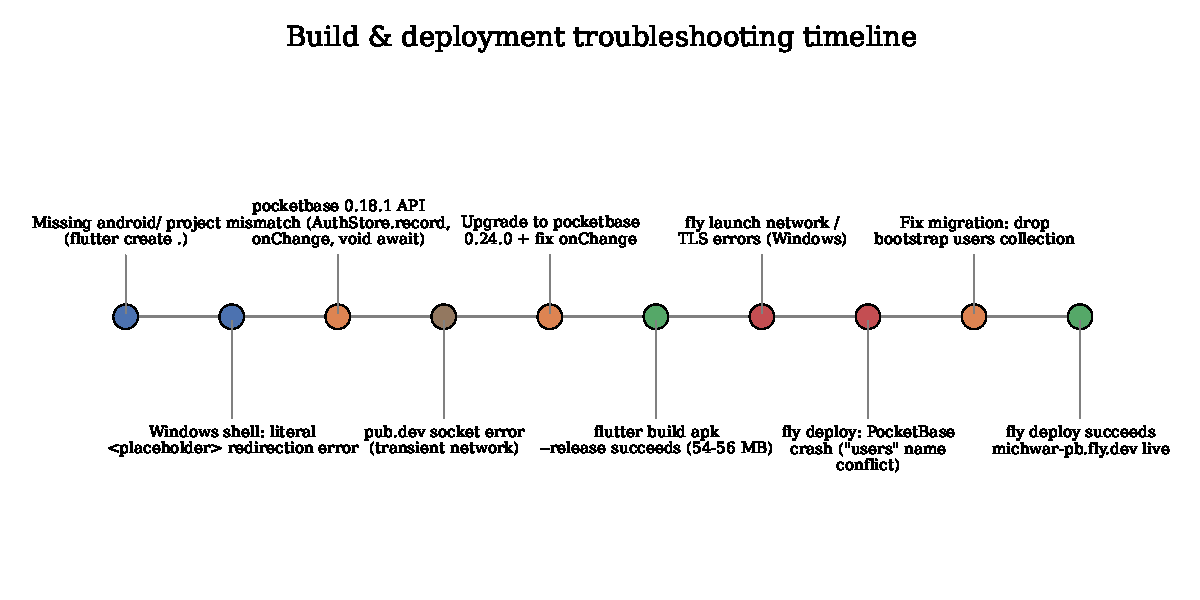
\includegraphics[width=\textwidth]{debug_timeline}
\caption{Chronological timeline of build and deployment issues, from the
initial \texttt{flutter build apk} attempt to the live Fly.io deployment.}
\label{fig:timeline}
\end{figure}

\begin{table}[htbp]
\centering
\caption{Build and deployment issues, causes, and resolutions}
\label{tab:issues}
\begin{tabular}{@{}p{3.4cm}p{4.3cm}p{4.6cm}@{}}
\toprule
\textbf{Symptom} & \textbf{Root cause} & \textbf{Resolution} \\
\midrule
\texttt{flutter build apk}: "The system cannot find the file specified" &
The project was authored without ever running \texttt{flutter create}, so
\texttt{android/} (and other platform folders) did not exist &
Ran \texttt{flutter create .} from the project root, which scaffolds platform
projects without touching \texttt{lib/} \\
\addlinespace
Same error persisted after scaffolding, with
\texttt{--dart-define=POCKETBASE\_URL=<...>} &
On Windows \texttt{cmd}, the literal \texttt{<}/\texttt{>} placeholder characters
in the example URL are interpreted as I/O redirection operators &
Substituted a real IP/URL with no angle brackets, e.g.\
\texttt{http://192.168.1.50:8090} \\
\addlinespace
Dart compile errors: \texttt{AuthStore.record} not defined,
\texttt{onChange} not invokable, \texttt{void} awaited &
\texttt{pocketbase} Dart SDK pinned at 0.18.1, whose \texttt{AuthStore} API
(\texttt{model}, callback-based \texttt{onChange}) differs from the
0.24.x API used by the ported code &
Bumped \texttt{pocketbase: \textasciicircum 0.18.1} $\rightarrow$ \texttt{\textasciicircum 0.24.0}; rewrote
\texttt{signOut} as \texttt{Future<void>}; rewrote
\texttt{authStateChanges()} to consume \texttt{AuthStore.onChange} as a
\texttt{Stream<AuthStoreEvent>} (Listing~\ref{lst:authservice}) \\
\addlinespace
\texttt{flutter pub get}: "Got socket error trying to find package pocketbase
at https://pub.dev" &
Transient network failure during dependency resolution &
Retried \texttt{flutter pub get}; succeeded on the second attempt \\
\addlinespace
\texttt{fly launch} / \texttt{fly deploy}: repeated
\texttt{read tcp ... wsarecv: A connection attempt failed},
\texttt{dial tcp ... connectex: A connection attempt failed},
\texttt{lookup api.fly.io: no such host} &
Intermittent connectivity from the Windows development machine to Fly's
API (consistent with TLS-inspecting antivirus/firewall or unstable
Wi-Fi/hotspot) &
Diagnosed via \texttt{Test-NetConnection api.fly.io -Port 443} (raw TCP
succeeded while HTTPS API calls failed); retried after switching network
and answering launch prompts with the documented values
(\texttt{n} to "tweak settings", \texttt{y} to "use this fly.toml") \\
\addlinespace
\texttt{fly deploy}: image built (18\,MB) and IPs provisioned, but
"\texttt{Error: timeout reached waiting for machine's state to change}" &
\texttt{fly logs} revealed the container itself crashed on boot:
\texttt{Failed to apply migration 1700000001\_users.js: name: Collection
name must be unique (case insensitive)} &
PocketBase $\geq$0.23 auto-creates a default \texttt{users} auth collection on
a fresh database; the migration now deletes this bootstrap collection
before creating the application's \texttt{users} collection
(Listing~\ref{lst:migration-users}) \\
\bottomrule
\end{tabular}
\end{table}

The final issue is the most architecturally significant: it was \emph{not} a
transient network problem despite occurring in the middle of a sequence of
genuine network issues, and it would have affected \textit{any} deployment
target (Fly.io, a VPS, a local Docker run against an empty volume), since it
is intrinsic to running the existing migrations against a PocketBase 0.23+
binary on a fresh database. Diagnosing it required separating "flyctl cannot
report status back to the Fly API" (a local network problem, visible as DNS
lookup failures for \texttt{api.fly.io} and \texttt{api.depot.dev}) from "the
container that Fly \textit{did} successfully start immediately exited" (an
application-level problem, visible only via \texttt{fly logs}, which showed
\texttt{pocketbase} printing the migration error and the init process exiting
with code 0 --- a "successful" exit from PocketBase's perspective after a
fatal startup error). \texttt{fly status} additionally showed the machine
state as \texttt{stopped}, confirming the container was not crash-looping but
had cleanly exited once.


% ===========================================================================
\section{Discussion}
\label{sec:discussion}
% ===========================================================================

\subsection{Architectural Trade-offs: Self-Hosting versus a Managed BaaS}

Migrating from Firebase to PocketBase trades a fully managed, infinitely
scalable (but billed-per-use and closed-source) backend for a single
self-contained binary that the project fully owns. The practical
consequences observed in this project are:

\begin{itemize}[nosep]
  \item \textbf{Operational simplicity at small scale.} The entire backend
    --- schema, business logic, file storage, and admin UI --- is a single
    18\,MB Docker image plus one SQLite file. Deployment to a free-tier
    Fly.io machine took a handful of commands and no managed-database
    provisioning.
  \item \textbf{Explicit, auditable business logic.} Every financially
    sensitive operation is a $\sim$30--130 line JavaScript function in
    \texttt{pb\_hooks/}, each wrapped in \texttt{\$app.runInTransaction()}. This
    is arguably \textit{more} auditable than a set of Firestore security
    rules plus separately deployed Cloud Functions, because the data model,
    the access rules, and the business logic all live in one repository and
    one runtime.
  \item \textbf{Scaling is now the operator's responsibility.} A single
    256\,MB shared-CPU machine and an embedded SQLite database are adequate
    for development and small-scale piloting, but horizontal scaling
    (read replicas, connection pooling, multi-region) would require
    additional engineering that a managed BaaS would otherwise absorb.
  \item \textbf{No vendor billing surprises.} The free Fly.io tier (3
    shared-cpu-1x VMs) comfortably hosts \texttt{michwar-pb} with
    \texttt{min\_machines\_running = 1}; there is no per-document-read or
    per-function-invocation billing to monitor.
\end{itemize}

\subsection{Robustness of the Transactional Hook Pattern}

A central design decision --- carried over faithfully from the original
Cloud Functions design --- is that \textit{no client write can directly
produce a billable number}. The \texttt{rides}, \texttt{wallets},
\texttt{wallet\_transactions}, and \texttt{drivers} financial fields all have
\texttt{update}/\texttt{delete} API rules of \texttt{null}, and the only way to
mutate them is through one of the seven \texttt{/api/michwar/...} hook routes,
each gated by \texttt{\$apis.requireAuth()} and wrapped in
\texttt{\$app.runInTransaction()}. This pattern provides two guarantees that
are difficult to achieve with purely declarative security rules: (1)
\textit{atomicity} across multiple collections (a completed ride atomically
updates \texttt{rides}, \texttt{drivers}, \texttt{wallets},
\texttt{wallet\_transactions}, and \texttt{users} in one transaction), and (2)
\textit{race-safety} for contended operations (the \texttt{/accept} route
re-checks \texttt{ride.driver} is still empty \textit{inside} the transaction,
so two drivers tapping "Accept" simultaneously cannot both succeed).

\subsection{Lessons Learned}

Several lessons emerged that generalize beyond this specific project:

\begin{enumerate}[nosep]
  \item \textbf{Pin and verify SDK versions against the server version they
    target.} The \texttt{pocketbase} Dart SDK's \texttt{AuthStore} API changed
    its shape (callback $\rightarrow$ stream, \texttt{model}
    $\rightarrow$ \texttt{record}) between 0.18.x and 0.24.x. Code written
    against one version fails to \textit{compile} (not just run) against the
    other, so a version bump must be treated as a small porting task, not a
    routine dependency update.
  \item \textbf{A framework's bootstrap behaviour can silently change.}
    PocketBase 0.23 began auto-provisioning a default \texttt{users} auth
    collection on first boot. Migrations written against an earlier
    assumption ("the database starts empty") must be defensive --- e.g.\
    check for and remove a colliding bootstrap collection before creating
    the application's own.
  \item \textbf{Separate "my tooling can't report status" from "my
    application failed."} The Fly.io deployment exhibited both a genuinely
    flaky local network connection \textit{and} a real application crash in
    the same deploy attempt. \texttt{fly status} (machine state) and
    \texttt{fly logs} (container stdout/stderr) were the tools that
    disambiguated the two; relying on \texttt{flyctl}'s own error message
    alone would have led to chasing the network issue indefinitely.
  \item \textbf{Windows shell quoting is a recurring trap for
    copy-pasted commands.} Placeholder syntax such as
    \texttt{<your-ip>} is idiomatic in documentation but is interpreted as
    redirection by \texttt{cmd.exe}/PowerShell, producing a misleading "file
    not found" error that has nothing to do with files.
  \item \textbf{\texttt{--dart-define} is an effective mechanism for
    environment-specific builds without source forks.} The same
    \texttt{lib/core/services/pocketbase\_service.dart} serves the emulator,
    LAN testing, and the public production URL, selected entirely at build
    time.
\end{enumerate}

\subsection{Limitations}

The system as deployed has several known limitations, documented in
\texttt{DEPLOYMENT.md}'s verification checklist:

\begin{itemize}[nosep]
  \item Push notifications (FCM) were intentionally dropped in favour of
    PocketBase realtime (SSE) subscriptions; \texttt{users.fcmTokens} remains
    an unused placeholder field for a future push provider.
  \item \texttt{POST /api/michwar/wallet/topup} currently credits a driver's
    wallet directly on call, which is appropriate for testing but must be
    placed behind a verified payment-provider webhook (e.g.\ CIB/EDAHABIA)
    before handling real money.
  \item The single 256\,MB Fly.io machine and embedded SQLite database are
    not designed for high-concurrency production traffic; horizontal scaling
    would require migrating to a server-based database (e.g.\ PostgreSQL,
    which PocketBase 0.23+ supports as an alternative to SQLite) and
    multiple machines behind Fly's load balancer.
  \item The live-trip-sharing feature (\texttt{live\_shares} collection) issues
    a public URL but assumes a separately hosted static tracking page; none
    was built as part of this work.
  \item Legacy Firebase artifacts (\texttt{.firebaserc}, \texttt{firebase.json},
    \texttt{firestore.rules}, \texttt{functions/}, etc.) remain in the repository
    as dead files pending manual removal.
\end{itemize}

\subsection{Future Work}

Natural extensions of this work include: (1) wiring a real payment
provider's webhook into \texttt{/api/michwar/wallet/topup}; (2) building the
live-trip-sharing static page described in \S\ref{sec:hooks}; (3) adding
automated integration tests against a disposable PocketBase instance
(e.g.\ in CI, spinning up the Docker image and exercising the
\texttt{/api/michwar/...} routes); (4) evaluating PocketBase's PostgreSQL
backend for higher-concurrency production use; and (5) building and
publishing iOS/web release artifacts alongside the Android APK, using the
same \texttt{--dart-define=POCKETBASE\_URL} mechanism.


% ===========================================================================
\section{Conclusion}
\label{sec:conclusion}
% ===========================================================================

This report has documented the complete migration of the MICHWAR
ride-hailing application's backend from Google Firebase to a self-hosted
PocketBase instance, and the subsequent build and public deployment of the
resulting system. The migration preserved the original architecture's
central guarantee --- that all financially sensitive state transitions are
computed and persisted atomically, server-side, inside transactions --- by
re-expressing the nine Firestore collections as PocketBase collections with
locked-down API rules, and the eight Cloud Functions as
\texttt{\$app.runInTransaction()} hook routes totalling roughly 1{,}400 lines
of JavaScript and migration code. The Flutter client (8{,}169 lines) required
only targeted changes: a new PocketBase service/auth layer, updated Riverpod
providers for SSE-based realtime subscriptions, and a dependency bump to
align with the PocketBase Dart SDK's 0.24.x \texttt{AuthStore} API. The
resulting Android release APK ($\approx$54\,MB) was successfully built and,
after diagnosing and fixing a PocketBase bootstrap-collection collision that
initially crashed the deployed container, the backend is now live at
\url{https://michwar-pb.fly.dev} on Fly.io's free tier --- giving MICHWAR a
fully self-owned, zero-recurring-cost backend that any downloaded APK can
reach from any network, with no manual configuration required by the end
user.


% ===========================================================================
\section*{References}
% ===========================================================================
\begin{enumerate}[nosep]
  \item PocketBase --- \textit{Open Source backend in 1 file}.
    \url{https://pocketbase.io/docs/}
  \item Flutter --- \textit{Build apps for any screen}.
    \url{https://docs.flutter.dev/}
  \item Riverpod --- \textit{A reactive caching and data-binding framework}.
    \url{https://riverpod.dev/}
  \item \texttt{go\_router} --- declarative routing package for Flutter.
    \url{https://pub.dev/packages/go_router}
  \item Fly.io --- \textit{Application platform for full stack apps}.
    \url{https://fly.io/docs/}
  \item \texttt{pocketbase} Dart SDK (v0.24.x).
    \url{https://pub.dev/packages/pocketbase}
  \item Niemeyer, G. \textit{Geohash}. \url{https://en.wikipedia.org/wiki/Geohash}
\end{enumerate}

\end{document}
\end{enumerate}

\end{document}
